% !TeX root = ../thuthesis-example.tex

\chapter{场景时延敏感度可感知的传输速率控制}
\section{本章序言}
云游戏是实时通信(Real-time communication,RTC)技术进步的产物,它通过将游戏渲染任务卸载到服务器,并将其以实时视频格式流式传输给用户,从而减轻了用户设备的计算负担。因此,云游戏对RTC所支持的实时传输和游戏画面流畅度提出了更高的要求,使得速率控制策略在确保用户体验质量方面至关重要。

现有的速率控制方法,如延迟排队理论建模\cite{arun2018copa,raeis2021queue}、固定规则\cite{ray2022sqp,carlucci2016analysis}、强化学习\cite{abbasloo2020classic,jay2019deep}以及基于用户感知的方法\cite{peng2023pacc,huang2023optimizing},主要目标是实现超低延迟。然而,它们通常忽视了云游戏中的延迟敏感性问题\cite{claypool2006latency,claypool2010latency}。考虑到延迟敏感性可以在流媒体画质\cite{shang2021study} 和端到端延迟之间提供更好的平衡,这对于确保令人满意的用户体验至关重要。在云游戏中,流媒体画质通过比特率、流畅度和画面抖动等指标进行衡量。

本章研究通过进行大规模数据测量和用户平均意见得分(Mean Opinion Score,MOS)实验,观察到了不同游戏场景中延迟对用户满意度的影响存在差异。某些依赖于实时决策的游戏类型在延迟增加时表现出满意度的显著下降,而其他类型的游戏在有限的延迟范围内则相对不受影响。为了描述这种现象,本章节引入了“敏感性”这一概念,用于描述延迟对用户参与度的影响,其中更高的敏感性表示在延迟上升时满意度下降得更为显著。本章节在多个游戏场景下的实验结果揭示了游戏可以被分为潜在的三种敏感性类别:高敏感、中敏感和低敏感。

为了便于在算法设计中应用这些发现,本章节利用最小二乘估计将MOS得分映射到延迟感知敏感性曲线。这些曲线建立了各个游戏类型的可接受延迟范围与延迟影响程度之间的关系,为带宽受限下的延迟和画质权衡提供了灵活性。

在追求这种权衡下的最佳用户体验(Quality of Experience,QoE)时,强化学习(Reinforcement Learning,RL)成为一种有效的解决方案。尽管已有十年的强化学习视频传输优化研究\cite{dao2022contemporary},但将强化学习应用于云游戏流媒体仍存在空白,特别是考虑到游戏延迟敏感性分类的问题。现有的研究,如ReCoCo\cite{markudova2023recoco}和R3Net\cite{fang2019reinforcement},未能考虑云游戏中不同游戏应用的敏感性差异。

为此,本章节提出了Sense,一种针对云游戏服务定制的演员-评论家(Actor-Critic)速率控制算法。与先前主要关注最小化传输延迟的方法不同,Sense 利用延迟感知敏感性曲线,在延迟和视觉保真度之间的权衡过程中提供更大的灵活性。通过基于空间感知信息(Spatial Information,SI) 和时间感知信息(Temporal Information,TI)确定的游戏类别选择奖励函数,Sense 提升了整体用户体验质量。通过结合延迟感知敏感性曲线并评估视觉流畅度和比特率,Sense能够学习最优策略,在权衡过程中最大化QoE。Sense的核心概念如图\ref{fig:teaser}所示,利用云游戏中的延迟感知敏感性差异,重新设计了强化学习的状态空间和奖励函数。对于云游戏平台上的游戏场景,Sense通过TI和SI确定其敏感性分类(高、中、低),然后选择相应的延迟感知敏感性曲线。通过整合延迟感知敏感性曲线,并考虑发送比特率和视觉流畅度等因素,Sense在不同游戏场景下实现了延迟和流媒体画质之间的更精细平衡。

\begin{figure}[h]
    \centering
    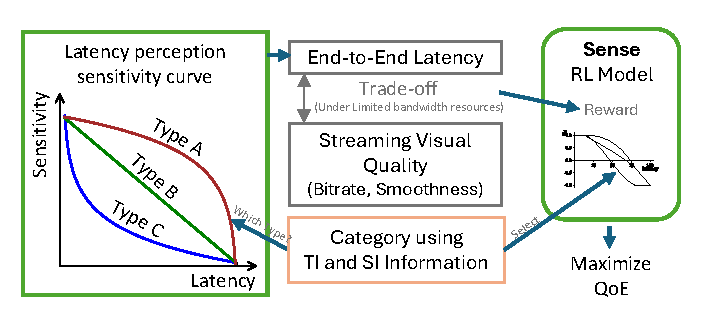
\includegraphics[width=0.78\textwidth]{figures/chap03/teaser.pdf}
    \caption{敏感度可感知的云游戏传输速率控制算法的设计框架}
    \label{fig:teaser}
\end{figure}

Sense的评估结果显示,它通过将延迟与各种场景类型对齐、减少画面抖动并准确分类场景敏感性,从而提高了QoE分数和场景分类准确性。

总结来说,本章节的贡献包括:
\begin{itemize}

\item 进行用户MOS实验,识别不同场景中的三种敏感性类型,并使用最小二乘估计拟合高、中、低敏感性的延迟感知敏感性曲线。
  
\item 提出Sense,一种专门为云游戏服务定制的Actor-Critic架构的强化学习速率控制算法。Sense在不同游戏场景中实现了延迟和画质之间的更好平衡,QoE提高了16.7\%。

\item 使用视频流信息(即时间感知信息TI和空间感知信息SI)对游戏场景的敏感性进行分类,准确率达到89.4\%,从而减少了对每个游戏的用户敏感性打分实验依赖。
\end{itemize}


\section{主客观测量实验和动机}
\subsection{数据测量与结果分析}\label{sec-measurement-study}
云游戏平台上有许多不同的场景和游戏。ClayPool等人的研究\cite{claypool2010latency}表明,游戏有不同的“阶段”,如“启动”、“同步”和“过渡”。这些阶段表现出显著的比特率差异,表明场景动态和延迟要求的变化。此外,不同的游戏类型,如第一人称射击游戏(First Person Shooting,FPS)、多人在线战术竞技场(Multiplayer Online Battle Arena,MOBA)、体育游戏(Sports Game)和集换式卡牌游戏(Collectible Card Game,CCG),在游戏过程中对延迟的敏感性各不相同。该研究还为不同的游戏提供了截止时间阈值。例如,射击游戏重度依赖于实时反应,而集换式卡牌游戏场景则优先考虑沉浸式体验,注重流畅的游戏过程和高质量的视觉效果。这些游戏的常见场景画面如图\ref{fig-game-sample}所示。
\begin{figure}[ht]
\centering
\begin{subfigure}[t]{0.4\linewidth}
  \centering
  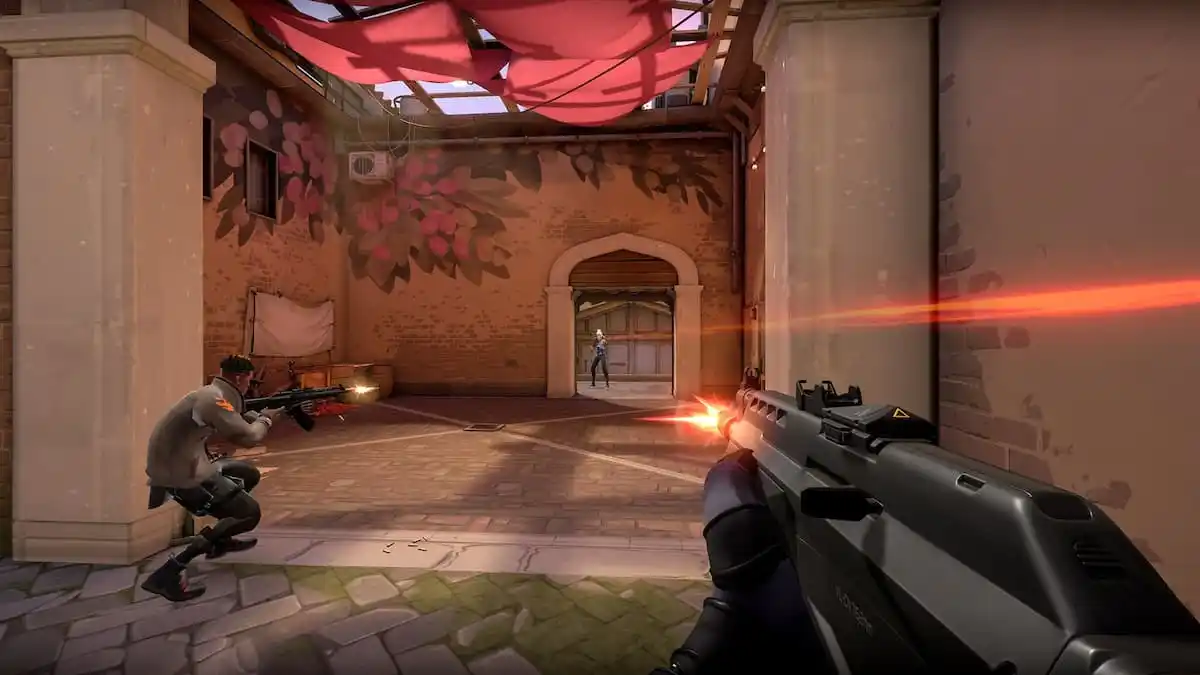
\includegraphics[width=\linewidth]{figures/chap03/game_example/fps_game.png}
  \caption{FPS 游戏}
  \label{fig-fps-game}
\end{subfigure}%
\begin{subfigure}[t]{0.4\linewidth}
  \centering
  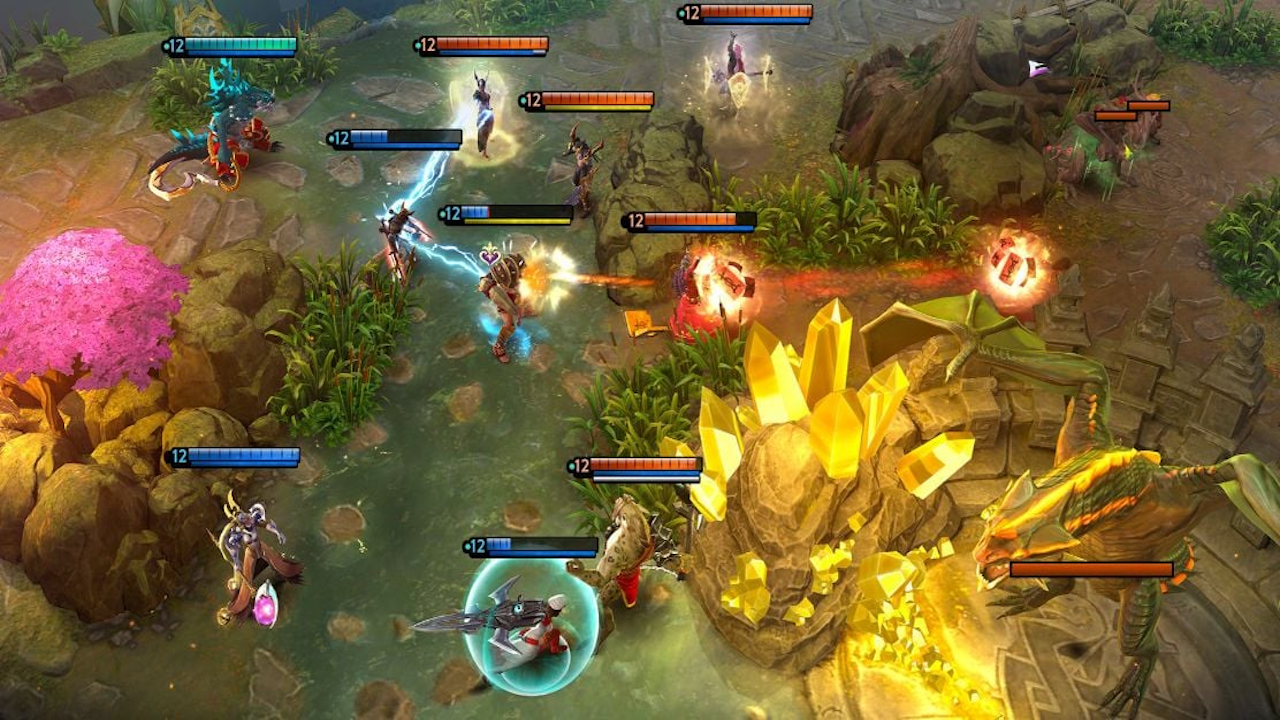
\includegraphics[width=\linewidth]{figures/chap03/game_example/moba_game.png}
  \caption{MOBA 游戏}
  \label{fig-moba-game}
\end{subfigure}

\begin{subfigure}[t]{0.4\linewidth}
  \centering
  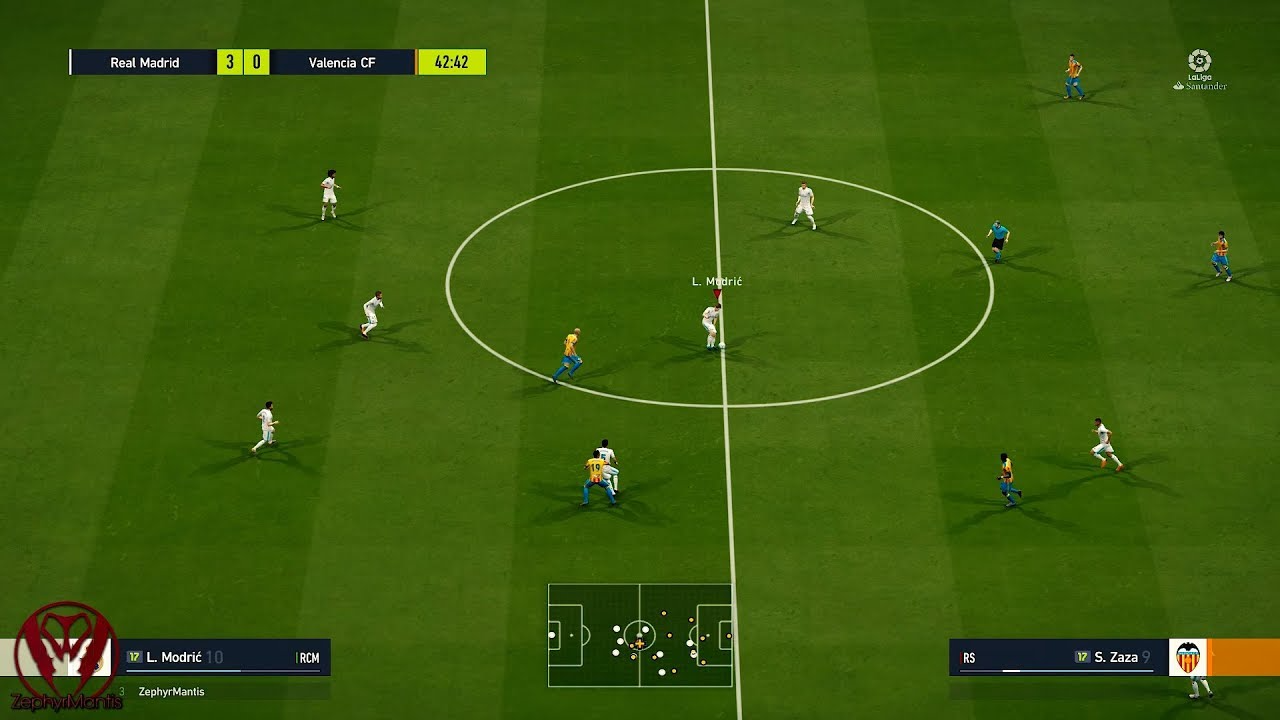
\includegraphics[width=\linewidth]{figures/chap03/game_example/sport_game.png}
  \caption{体育游戏}
  \label{fig-sport-game}
\end{subfigure}%
\begin{subfigure}[t]{0.4\linewidth}
  \centering
  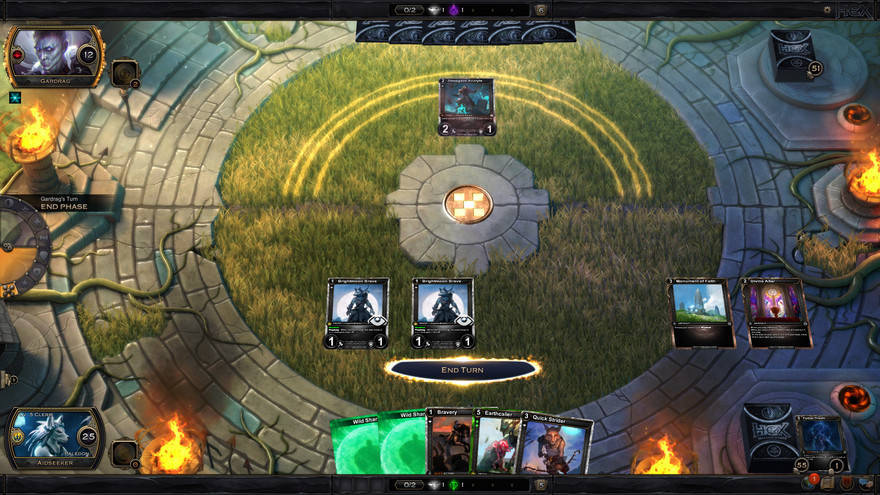
\includegraphics[width=\linewidth]{figures/chap03/game_example/chess_game.png}
  \caption{集换式卡牌游戏}
  \label{fig-chess-game}
\end{subfigure}

\caption{不同类型游戏的常见场景示例}
\label{fig-game-sample}
\end{figure}


\subsubsection{系统运行架构和时间延迟测量方式}
云游戏将渲染和其他计算密集型处理过程转移到强大的云服务器上,并将渲染后的视频流传输到用户设备,类似于视频流服务的工作方式。此外,云游戏还包括实时的用户交互。因此,衡量用户在云游戏中感知到的延迟的一个关键方式是使用“操作到画面”(Motion-to-Photon,MTP)延迟。延迟的主要来源如图\ref{fig_system_architecture}所示。

\begin{figure} [ht]
\centering
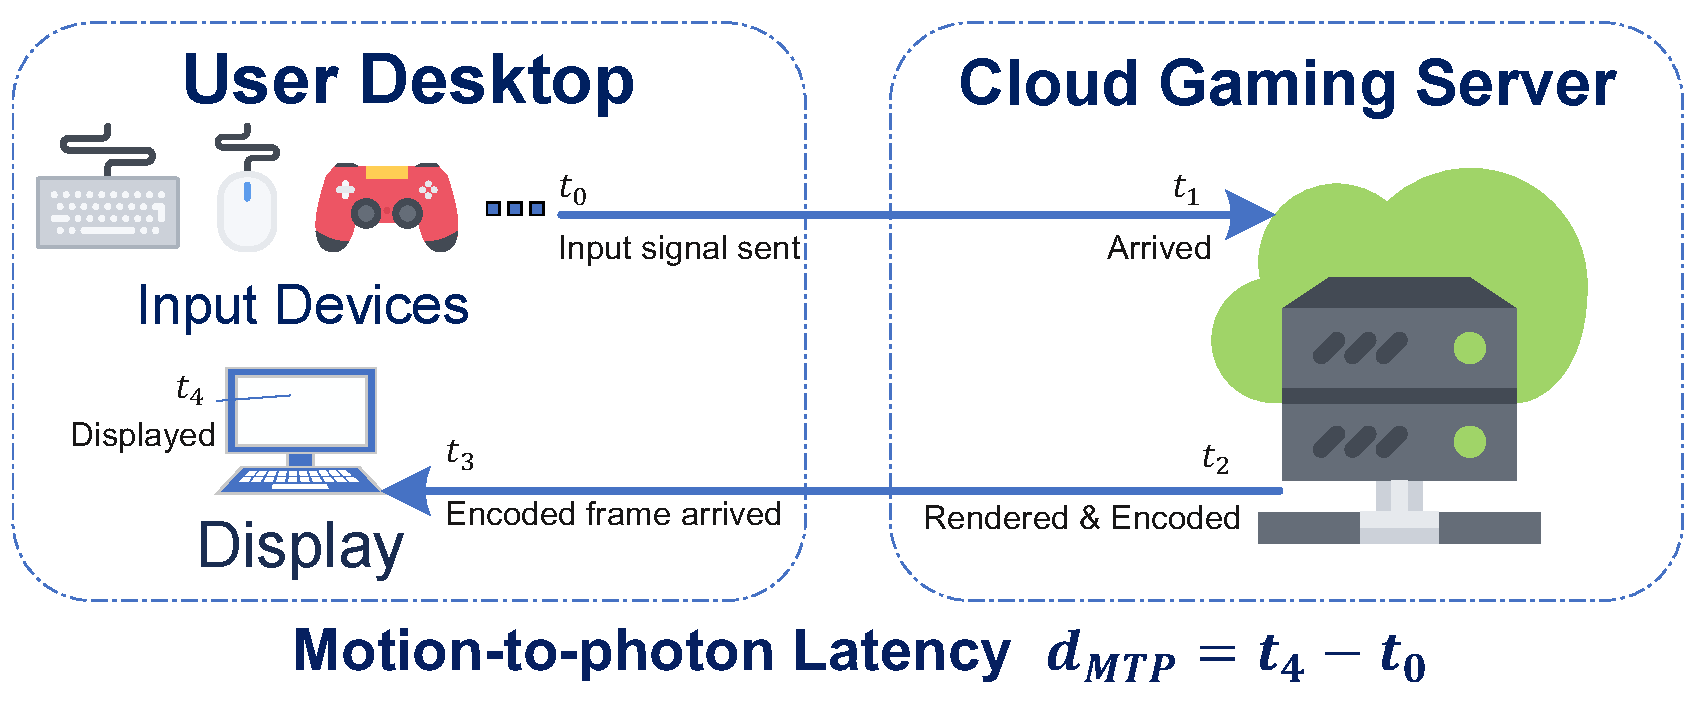
\includegraphics[width=0.7\textwidth]{figures/chap03/system_architecture.pdf} 
\caption{云游戏实时通信系统的架构及时刻}
\label{fig_system_architecture}
\end{figure}

一旦用户在时间 $t_0$ 触发操作,请求会由于网络延迟在时间 $t_1$ 到达服务器。服务器完成游戏画面的渲染并使用低延迟编码器进行编码,编码在时间 $t_2$ 完成。然后,数据包到达用户设备并在时间 $t_3$ 解码。最后,视频流完全解码并显示在用户屏幕上,时间为 $t_4$。MTP 延迟考虑了从 $t_0$ 到 $t_4$ 的整个处理延迟,并定义为 $d_{MTP} = t_4 - t_0$,即用户执行操作与该操作显示在屏幕上的时间差。这种方法提供了用户感知的延迟的更准确测量,从而更精确地评估云游戏中的QoE。

\subsubsection{大规模数据测量}
为了研究不同应用在云游戏实时通信平台上对延迟效应的QoE敏感性,本工作在一个商业平台上进行了为期一年的大规模测量研究。数据集包含超过350万条验证记录,最细粒度为单个连接的建立到终止的过程。为了减少真实生产环境中可能出现的混杂因素的影响,本工作采用了多个标准来筛选大量在线数据,包括由用户发起但没有后续活动的连接,以及持续时间过短的连接。被测量的游戏及每款游戏使用的数据集如表\ref{table_flow_count}所示。数据有两种不同粒度类型:流粒度持续时间是指从用户发起连接请求开始,直到用户关闭连接为止,形成一组统计数据为一次统计,作为单条数据进行使用的数据;而帧粒度持续时间则是指单个流中每一帧画面显示为一次统计,一个流形成一张表格。后者的粒度比前者更细,可以获得更多细节统计信息,收集用于进一步探索,两者共同使用形成测量结果。

\begin{table}[ht]
\centering
\caption{用于统计游戏的流属性统计}
\begin{tabular}{@{}ccccc@{}}
\toprule
\textbf{游戏}        & \textbf{流粒度持续时间(小时)} & \textbf{帧粒度持续时间(小时)} \\ \midrule
2D-RPG I             & 3707.74                  & 910.23                    \\
2D-RPG III           & 2558.73                  & 460.17                    \\
3D-RPG I             & 889.68                   & 49.83                     \\
动作游戏 I           & 1194.60                  & 102.73                    \\
A-RPG I              & 529.15                   & 87.37                     \\
休闲游戏 I           & 70.47                    & 3.29                      \\
CCG I                & 200.42                   & 12.80                     \\
FPS I                & 1360.89                  & 277.21                    \\
FPS II               & 151.32                   & 79.51                     \\
FPS III              & 570.81                   & 62.75                     \\
FPS IV               & 281.95                   & 20.71                     \\
MMORPG I             & 638.79                   & 82.72                     \\
MOBA I               & 685.65                   & 378.66                    \\
MOBA II              & 247.16                   & 98.07                     \\
运动游戏 I           & 1068.06                  & 249.90                    \\
运动游戏 II          & 155.76                   & 35.31                     \\
运动游戏 III         & 1376.29                  & 0.13                      \\
TPS I                & 331.30                   & 25.43                     \\ \bottomrule
\end{tabular}
\label{table_flow_count}
\end{table}



从大规模测量中获得的原始数据,由于记录中存在异常使用数据,往往偏离理想数据。为了确保数据测量的准确性,需要应用某些规则,尽可能排除由于用户或设备链路问题导致的异常数据。可能的异常数据情况包括:
\begin{itemize} 
\item \textbf{用户提前退出:}该情况指的是用户与服务器建立连接后,但未实际进行游戏便退出。此类连接通常持续时间较短,不超过 2 分钟。 

\item \textbf{僵尸流量:}该情况指的是客户端与服务器的连接异常断开,但流量未停止并继续计数,导致数据不正确。这样可能导致流量被计量几个小时甚至超过一天,超过了正常可接受的长时间使用时长。 

\item \textbf{频繁切换网络:}为了排除用户网络连接不稳定的情况,测量中选择常见的网络类型(2.4GHz 和 5GHz Wi-Fi、以太网或蜂窝数据)。在单次连接中,频繁切换网络连接的情况将不被纳入统计。 

\item \textbf{极低的实际编码比特率:}实际编码比特率低于设置比特率的十分之一,通常是由于长时间静态或极小的画面,导致需要传输的残余信息非常少,从而导致极低的比特率。这表明尽管用户已连接,但并未进行任何操作。 

\item \textbf{低交互频率}:用户客户端接收到的输入频率极低,如键盘、鼠标或游戏手柄的输入频率。此类情况也表明用户已建立连接,但未进行任何游戏活动。 

\item \textbf{异常的客户端处理时间:}通常,在性能稳定的机器上接收和解码视频不应超过某个时间限制。处理时间波动较大或连接时间过长的情况也应排除。在处理延迟过高的情况下,用户无法正常游戏,而连接时间过长则表明客户端存在异常行为,因此需要排除。 

\end{itemize}

游戏选择包括平台上的九款主流热门游戏:第一人称射击(First Person Shooting,FPS)游戏I、II、III,2D角色扮演(RPG)游戏I、II,体育游戏I,集换式卡牌游戏(Collectible Card Game,CCG)I,以及多人在线战术竞技(Multiplayer Online Battle Arena,MOBA)游戏I、II。这些热门游戏具有大量数据流量,并涵盖了传统意义上不同类型和类别的游戏,代表了不同游戏应用在云游戏实时通信系统上的差异。

不同类型游戏对MTP延迟的敏感性如图\ref{fig-real-measurement-results-High-Delay-Sensitivity-Games}、\ref{fig-real-measurement-Medium-Delay-Sensitivity-Games} 和 \ref{fig-real-measurement-results-Low-Delay-Sensitivity-Games} 所示。为了反映用户参与度,测量选择使用时间作为主要指标,研究MTP延迟与用户参与度之间的关系。由于游戏时长可能受关卡设计或回合时长等因素的影响,测量对游戏时长进行了归一化处理。归一化过程包括计算每个游戏的平均使用时间,并与单个游戏回合的典型时长进行验证。如果平均使用时间明显短于单个游戏回合所需的最小时长,则认为数据存在混杂因素,并进一步进行筛选。确认正确的平均使用时间后,所有测得的使用时间将除以上述平均值,得到相对于平均游戏使用时间的百分比。通过这种方式,每个游戏的标准使用时间在y轴上归一化为1.0x,从而更容易观察相对时长。游戏被分为三类:高敏感度、中敏感度和低敏感度游戏。随着MTP延迟的增加,图\ref{fig-real-measurement-results-High-Delay-Sensitivity-Games} 中的三类游戏的游玩时长表现出初期的指数级下降,而图\ref{fig-real-measurement-Medium-Delay-Sensitivity-Games} 中则呈现更接近线性的下降,不同游戏的时长下降至0.6 - 0.8x。相比之下,图\ref{fig-real-measurement-results-Low-Delay-Sensitivity-Games} 中的游戏在某一延迟阈值(大约35ms)之前,游玩时长没有显著下降,超过该阈值后,游玩时长降至0.8x - 0.95x。
\begin{figure}[htbp]
\centering
\begin{subfigure}[t]{0.4\linewidth}
  \centering
  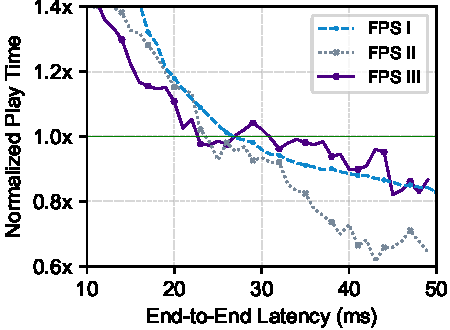
\includegraphics[width=\linewidth]{figures/chap03/measurement_data/delay-sensitive.pdf}
  \caption{高敏感度游戏}
  \label{fig-real-measurement-results-High-Delay-Sensitivity-Games}
\end{subfigure}%
\begin{subfigure}[t]{0.4\linewidth}
  \centering
  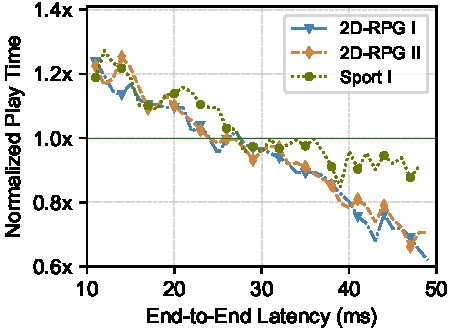
\includegraphics[width=\linewidth]{figures/chap03/measurement_data/delay-linear-sensitive.pdf}
  \caption{中敏感度游戏}
  \label{fig-real-measurement-Medium-Delay-Sensitivity-Games}
\end{subfigure}

\begin{subfigure}[t]{0.4\linewidth}
  \centering
  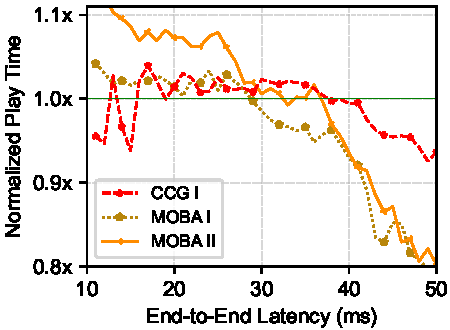
\includegraphics[width=\linewidth]{figures/chap03/measurement_data/delay-not-sensitive.pdf}
  \caption{低敏感度游戏}
  \label{fig-real-measurement-results-Low-Delay-Sensitivity-Games}
\end{subfigure}%
\begin{subfigure}[t]{0.4\linewidth}
  \centering
  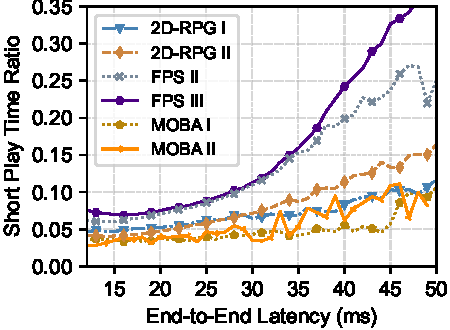
\includegraphics[width=\linewidth]{figures/chap03/measurement_data/early_quit_ratio.pdf}
  \caption{短时游玩比例}
  \label{fig-real-measurement-results-Short-Play-Time-of Games}
\end{subfigure}

\caption{不同敏感度的游戏在平均时延下的使用时长}
\label{fig:measurement-result}
\end{figure}


由于大多数游戏要求用户参与实时游戏,且无法像观看视频那样随意退出,因此使用像 \cite{chengrebuffering} 中的退出率已经不再可靠。测量中定义了短时游戏时长的概念,并将每个游戏的平均游戏时长的50\%作为短时游戏时长的阈值。在图\ref{fig-real-measurement-results-Short-Play-Time-of Games} 中,测量观察了在不同平均延迟条件下,用户进行短时游戏时长的概率。可以看出,高延迟敏感游戏的退出率随着延迟的增加显著加快,而中低延迟敏感游戏的退出率增长大约在5\%到10\%之间,低延迟敏感游戏的影响略小。


有趣的是,当直接绘制原始数据时,可以从测量结果中观察到因素之间呈现出非单调关系,这与 \cite{balachandran2013developing} 中的测量结果非常相似,在特定的延迟值处存在多个峰值。在数据过滤后,这一趋势变得不那么显著,但仍然存在,确认了这一非单调关系的出现是由于频繁的延迟波动导致了平均延迟的下降和QoE的下降。

\subsection{用户MOS实验}\label{sec-mos}

测量实验说明了游戏敏感度的区分可分为高、中、低三个敏感度。为了进一步研究不同场景下延迟差异和用户满意度要求,研究开展了在不同场景下的平均意见得分(MOS)评分测试,以评估用户在特定延迟条件下的满意度水平。实验包括20名参与者,他们的画像如表\ref{tab:userinfo}所示。

\begin{table}[ht]

\caption{参与者的基本信息}
\renewcommand\arraystretch{1.25}

\begin{center}

\begin{tabular}{@{}ccccc@{}}
\toprule
\multicolumn{2}{c}{游戏类型}                       & FPS & \begin{tabular}[c]{@{}c@{}}MOBA 和 CCG\end{tabular} & \begin{tabular}[c]{@{}c@{}}RPG 和 体育\end{tabular} \\ \midrule
\multicolumn{2}{c}{参与者人数}                   & 5   & 9                                                  & 6                                                   \\ \hline
\multirow{3}{*}{年龄}                & 18-22岁    & 2   & 4                                                  & 2                                                   \\
                                 & 23-26岁    & 2   & 3                                                  & 2                                                   \\
                                 & 27-30岁    & 1   & 2                                                  & 2                                                   \\ \hline
\multirow{3}{*}{游戏经验}          & 初学者     & 1   & 1                                                  & 1                                                   \\
                                 & 中级       & 2   & 4                                                  & 3                                                   \\
                                 & 高级       & 2   & 4                                                  & 2                                                   \\ \bottomrule
\end{tabular}
\end{center}
\label{tab:userinfo}
\end{table}


共获得220条有效记录,且没有引发伦理问题。为了模拟网络连接中的端到端延迟,实验使用了 NetEm 和 TC(流量控制)在服务器和用户设备之间建立了专用网络连接。在预定义的时间间隔内,用户提供了5分制MOS评分,反映他们的游戏体验。MOS评分为3被设定为用户满意或不满意的临界值。具体的MOS评分含义包括在了表\ref{tab:mos_rate}中。

\begin{table}[ht]
    \caption{用户MOS评分值的含义}
    \renewcommand\arraystretch{1.25}
    \centering
    \begin{tabular}{@{}cc@{}}
\toprule
评分 & 含义                                                           \\ \midrule
5     & 高清晰度和平滑画面,非常即时的响应。                          \\
4     & 相当清晰和平滑的画面,较为即时的响应。                        \\
3     & 平均视觉质量,满足最低响应要求。                              \\
2     & 画面有些卡顿和延迟,响应不够即时。                            \\
1     & 无法接受的视觉质量,响应缓慢影响游戏体验。                   \\ \bottomrule
\end{tabular}
    \label{tab:mos_rate}
\end{table}


调查结果的平均值如图\ref{fig-average-user-mos-rating}所示,将游戏分为高、中、低三种敏感性类别。结果显示,不同游戏类型对增加的端到端延迟的敏感性各不相同。这一发现表明,可以将原本用于减少延迟的资源重新分配到在带宽受限的情况下提升视觉质量。通过在延迟和视觉质量之间进行平衡,云游戏平台可以优化资源分配,改善整体游戏体验,特别是在延迟不那么关键的场景中。
\begin{figure}[ht]
\centering
\begin{subfigure}[t]{0.49\linewidth}
  \centering
  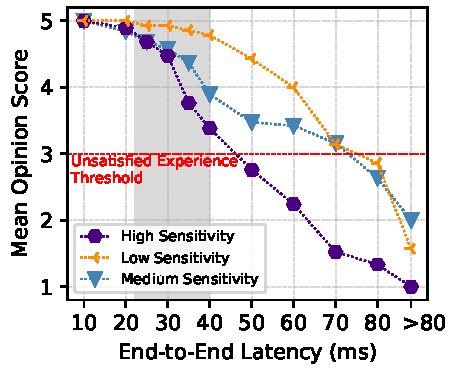
\includegraphics[width=\linewidth]{figures/chap03/latency_curve/user_perception.pdf}
  \caption{用户平均MOS评分}
  \label{fig-average-user-mos-rating}
\end{subfigure}%
\begin{subfigure}[t]{0.49\linewidth}
  \centering
  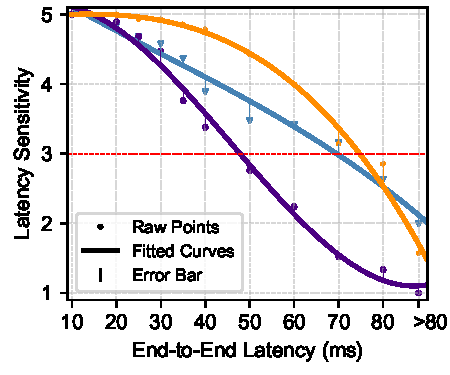
\includegraphics[width=\linewidth]{figures/chap03/latency_curve/fitted_curve.pdf}
  \caption{拟合曲线}
  \label{fig-fitted-curves}
\end{subfigure}

\caption{用户MOS评分实验结果和数值拟合结果}
\label{fig-latency-curve}
\end{figure}



\subsection{测量结果使用方案和设计挑战}
利用云游戏平台中不同应用的延迟敏感性为流媒体传输中的发送速率适应性调整提供了机会,从而在延迟和视觉质量之间实现更好的平衡,最终提升用户体验质量。然而,目前云游戏平台如何将测量结果揭示的敏感性特征融入其速率控制算法中仍存在空缺。弥补这一空缺需要克服若干挑战。

\textbf{挑战一:敏感性的量化。} 虽然实验结果提供了关于不同游戏场景对延迟敏感性的定性见解,但缺乏一种系统化、可量化的度量方法,使得延迟对用户体验的具体影响难以直接衡量。开发一个感知函数来评估敏感性水平对于实现这一目标至关重要。该函数应该能够以形式化的数学表达准确反映延迟对用户体验的实际影响,进而将其映射到算法的设计中。

\textbf{挑战二:速率控制算法的设计。} 在不同的游戏场景下,延迟与视觉质量的平衡关系存在较大差异,因此所设计的速率控制算法必须能够自适应地适应不同延迟敏感性需求,而通过自适应学习在波动的网络条件下实现最大化用户体验质量的最终目标是一项复杂的决策任务。

\textbf{挑战三:确定场景延迟敏感性。} 不同的应用场景对延迟的敏感程度各不相同,如何基于客观指标准确地确定当前场景的敏感性分类对于最终的框架设计和实施至关重要。

\section{时延敏感性曲线拟合分析}\label{sec-latency-curve} 
通过进行MOS评分实验,本实验获得了在不同延迟值下,用户的平均评分 $r_j$ 和对应的延迟值 $d_j$,如式\eqref{eq:djrj}所示: 
\begin{equation}
\begin{aligned}
    (d_j, r_j),  j= 1, 2, ..., m.
\end{aligned}
\label{eq:djrj}
\end{equation}

本章节利用最小二乘估计(Least Square Estimate,LSE)对特定延迟下的平均用户评分进行回归分析,从而得到拟合的延迟感知敏感度曲线。
令 $f(d)$ 是一个在 $m+1$ 个节点上定义的离散函数,其中 $a = d_0 < d_1 < \dots < d_m = b$,即 $f(d)$ 由式\eqref{eq:point}表示的点组成:
\begin{equation}
\begin{aligned}
    (d_j, f(d_j) = r_j),  j= 1, 2, ..., m.
\end{aligned}
\label{eq:point}
\end{equation}
$d_j$ 表示系统的端到端延迟,$r_j = f(d_j)$ 表示用户的 MOS 评分。同时,有一组在区间 $[a,b]$ 上定义的线性无关函数 $\varphi_0(d), \varphi_1(d), ..., \varphi_n(d)$,它们构成了 $\Phi = span\{\varphi_0, \varphi_1, ..., \varphi_n\}$。

为了拟合 $f(d)$,使用了LSE来得到最优化的函数 $s^* \in \Phi$,使得满足式\eqref{eq:satsify}的条件:
\begin{equation}
\begin{aligned}
    \sum^{m}_{j=0}[f(d_j)-s^*(d_j)]^2 = \min_{s \in \Phi} \sum^{m}_{j=0}[f(d_j)-s(d_j)]^2,
\end{aligned}
\label{eq:satsify}
\end{equation}
由于 $s \in \Phi$,可以表示 $s(d) = \sum^{n}_{i=0}a_i\varphi_i(d)$。这个问题现在转化为寻找式\eqref{eq:minpro}所示函数的最小值:
\begin{equation}
\begin{aligned}
    F(a_0, a_1, ..., a_n) = \sum^{m}_{j=0}\left[f(d_j)-\sum^{n}_{i=0}a_i\varphi_i(d_j)\right],
\end{aligned}
\label{eq:minpro}
\end{equation}
而$F(a_0, a_1, ..., a_n)$ 达到最小值的必要条件如式\eqref{eq:conddi}所示。
\begin{equation}
\begin{aligned}
    \frac{\partial F}{\partial a_k} = -2\sum^{m}_{j=0}\left[f(d_j)-\sum^{n}_{i=0}a_i\varphi_i(d_j)\right]\varphi_k(d_j)= 0, k = 0, 1, ..., n.
\end{aligned}
\label{eq:conddi}
\end{equation}


现定义式\eqref{eq:condi}:
\begin{equation}
\begin{aligned}
(\varphi_i,\varphi_k) =& \sum^{m}_{j=0}\varphi_i(d_j)\varphi_k(d_j),\\ 
(f,\varphi_k) =& \sum^{m}_{j=0}f(d_j)\varphi_k(d_j),
\end{aligned}
\label{eq:condi}
\end{equation}
可以将式\eqref{eq:condi}简化为式\eqref{eq:simple}:
\begin{equation}
\begin{aligned}
\sum^{n}_{i=0}(\varphi_i,\varphi_k)a_i = (f,\varphi_k), k = 0, 1, ..., n.
\end{aligned}
\label{eq:simple}
\end{equation}
这是一个非齐次线性方程组,当系数矩阵非奇异时,可以解出式\eqref{eq:mat}:
\begin{equation}
\begin{aligned}
\begin{bmatrix}  
  (\varphi_0,\varphi_0) & (\varphi_0,\varphi_1) & \cdots & (\varphi_0,\varphi_n) \\  
  (\varphi_1,\varphi_0) & (\varphi_1,\varphi_1) & \cdots & (\varphi_1,\varphi_n) \\  
  \vdots & \vdots & \ddots & \vdots \\  
  (\varphi_n,\varphi_0) & (\varphi_n,\varphi_1) & \cdots & (\varphi_n,\varphi_n)  
\end{bmatrix} \begin{bmatrix}  
   a_0 \\  
  a_1 \\  
  \vdots \\  
  a_n  
\end{bmatrix}  = \begin{bmatrix}  
   (f,\varphi_0) \\  
  (f,\varphi_1) \\  
  \vdots \\  
  (f,\varphi_n)
\end{bmatrix}.\end{aligned}
\label{eq:mat}
\end{equation}

对于用户评分数据,拟合过程选择使用最小二乘法拟合三次多项式、四次多项式、指数函数和对数函数。三次多项式的拟合结果获得了最小的误差,分别对应于三条灵敏度曲线,如图\ref{fig-fitted-curves} 所示。该曲线可以用式\eqref{eq:expr}表示:
\begin{equation}
\begin{aligned}
r = a_3 \cdot d^{3} + a_2 \cdot d^{2} + a_1 \cdot d + a_0,
\end{aligned}
\label{eq:expr}
\end{equation}
其中 $a_j$ 如表\ref{tab:a3a2a1a0}所示。


\begin{table}[ht]
\caption{使用三次多项式拟合用户评分的多项式系数}
\renewcommand\arraystretch{1.25}
\centering
% \resizebox{0.6\columnwidth}{!}{%
\begin{tabular}{@{}ccccc@{}}
\toprule
\textbf{}                              & \textbf{$a_3$}          & \textbf{$a_2$}          & \textbf{$a_1$}         & \textbf{$a_0$} \\ \midrule
\multicolumn{1}{c|}{\textbf{高敏感性}}  & $1.498 \times 10^{-5}$   & $-2.075 \times 10^{-3}$   & $2.130 \times 10^{-2}$  & $5.088$        \\

\multicolumn{1}{c|}{\textbf{中敏感性}} & $- 2.060 \times 10^{-6}$ & $1.863 \times 10^{-4}$   & $-3.862 \times 10^{-2}$ & $5.480$        \\
\multicolumn{1}{c|}{\textbf{低敏感性}}  & $- 4.580 \times 10^{-6}$ & $- 6.599 \times 10^{-5}$ & $4.117 \times 10^{-3}$  & $4.973$        \\ \bottomrule
\end{tabular}
% }
\label{tab:a3a2a1a0}
\end{table}


\section{场景需求可感知传输速率控制算法设计}
本章节中阐述了一个基于 Actor-Critic 架构的强化学习速率控制算法的设计,该算法利用延迟感知敏感度曲线为云游戏平台上的不同场景提供不同的速率调整策略。为了应对场景的敏感度分类问题,本章节利用了视频的空间感知信息(Spatial Information,SI) 和时间感知信息(Temporal Information,TI) 提供的信息来解决这一问题。

\subsection{感知强化学习空间设计}\label{sec:rl-design}
将强化学习的概念应用于速率控制问题,可以将网络视为观察环境,代理则根据当前的网络状态做出发送速率的决策。设定了一个固定的时间间隔 $\Delta t$ 为 200 毫秒,用于观察和决策。实验重新设计了强化学习的状态空间和动作空间。奖励函数由延迟、视频流畅度和与网络相关的指标组成,这些指标能够反映视觉质量和用户体验的质量。

\subsubsection{状态空间}
状态空间由网络状态的历史统计值构成。网络在固定时间间隔 $\Delta t = 200$ 毫秒内收集以下状态信息:(i)平均接收速率 $RR$,计算为每毫秒内所有接收数据包负载字节的总和的平均值;(ii)平均端到端延迟 $D$;(iii)数据包丢失率 $L$;(iv)帧间到达时间序列 $J$;(v)上一步采取的动作 $a$,即 $\boldsymbol{s_t} = (RR_t, D_t, L_t, J_t, a_t)$。选择过去 5 个值作为状态向量的组成部分,这对应于过去一秒钟的记录:$\mathcal{S}t = (\boldsymbol{s_t}, \boldsymbol{s{t-1}}, ..., \boldsymbol{s_{t-4}})$。


\subsubsection{动作空间}
动作空间设置为每个时间周期内发送速率的决策值。决策值可以选择在 $[3, 50]$ Mbps 范围内,以确定传输速率。为了在训练过程中保持性能稳定,实验设计使用对数函数将发送速率 $R_s$ 的范围归一化到 $[0, 1]$,如式\eqref{eq:logsend}所示:

\begin{equation}
\begin{aligned}
    R_{slog} = \frac{\log(R_s)-\log(R_{min})}{\log(R_{max})-\log(R_{min})}.
\end{aligned}
\label{eq:logsend}
\end{equation} 

\subsubsection{奖励函数}
奖励函数同时考虑了延迟和视觉质量,这两者对体验质量有显著影响。它由以下几个部分组成:(i) 平均端到端延迟的奖励 $R_d$,(ii) 屏幕卡顿或抖动的奖励 $R_j$,(iii) 丢包率的奖励 $R_l$,(iv) 带宽利用率的奖励 $R_u$。其中,丢包率和带宽利用率是影响视觉质量和延迟的关键因素。当丢包严重时,解码器可能无法及时呈现完整的帧内容,导致帧不完整或卡顿。带宽利用率反映了在有限带宽下的可用比特率,它影响视频内容的分辨率和量化级别。奖励函数的所有组成部分都被归一化到 $[-1, 1]$ 范围内。奖励函数构成的完整示意图如图\ref{fig:reward-function}所示。

\begin{figure}[ht]
\centering
\begin{subfigure}[t]{0.5\linewidth}
  \centering
  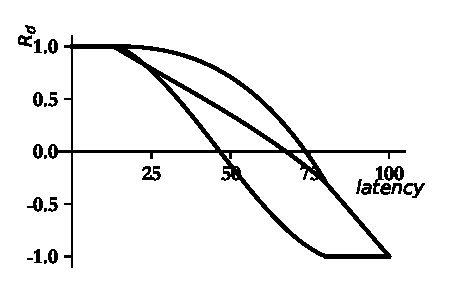
\includegraphics[width=\linewidth]{figures/chap03/reward_function/Rd.pdf}
  \caption{延迟奖励}
  \label{fig:Latency Reward}
\end{subfigure}%
\begin{subfigure}[t]{0.5\linewidth}
  \centering
  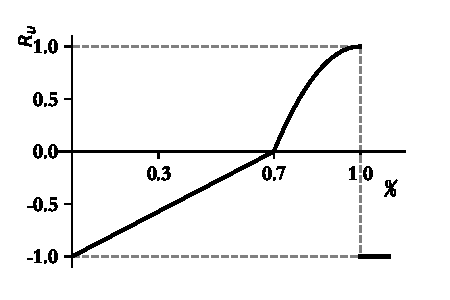
\includegraphics[width=\linewidth]{figures/chap03/reward_function/Ru.pdf}
  \caption{带宽利用率奖励}
  \label{fig:Bandwidth Utilization Reward}
\end{subfigure}

\begin{subfigure}[t]{0.5\linewidth}
  \centering
  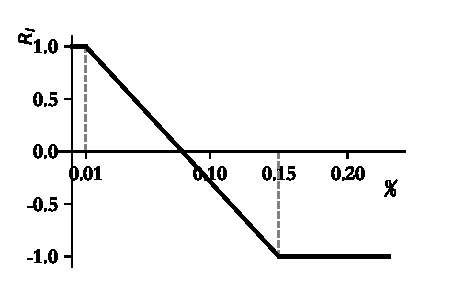
\includegraphics[width=\linewidth]{figures/chap03/reward_function/Rl.pdf}
  \caption{丢包率奖励}
  \label{fig:Loss Ratio Reward}
\end{subfigure}%
\begin{subfigure}[t]{0.5\linewidth}
  \centering
  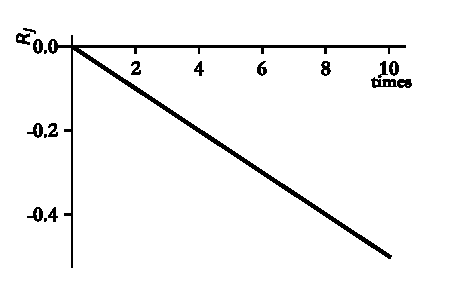
\includegraphics[width=\linewidth]{figures/chap03/reward_function/Rj.pdf}
  \caption{屏幕抖动奖励}
  \label{fig:jitter Reward}
\end{subfigure}

\caption{强化学习中的奖励函数构成}
\label{fig:reward-function}
\end{figure}





平均端到端延迟奖励 $R_d$ 将每个延迟感知敏感度曲线映射到相应的延迟奖励函数,如图\ref{fig:Latency Reward} 所示。对于超出范围的值,使用线性函数。在给定的游戏应用中,选择与其敏感性特征相对应的敏感度曲线作为奖励函数。三条曲线的表达式如式\eqref{eq:rd} 所示:
\begin{equation}
\begin{aligned}
R_{d} = 
    \begin{cases}
        1 & d < 10\\
        min\{1,0.5 \times r(d) - 1.55 \}& 10 \leq d \leq 85 \\
        max\{-1,- 0.035d +2.507\} & d > 85\\
\end{cases}
\end{aligned}
,
\label{eq:rd}
\end{equation}
其中 $r(d)$ 是式\eqref{eq:expr}所表示的内容。最终的奖励值为 $r(d)$,其中根据场景的敏感度类别选择三条曲线中的一条。

带宽利用率奖励 $R_u$ 考虑了流媒体传输流使用的带宽与总可用带宽的比率。设置传输速率过低会导致资源浪费和视频质量下降,从而造成次优的用户体验(QoE);而设置速率过高则可能导致缓冲积累,从而增加延迟。因此,带宽利用率的设计如图\ref{fig:Bandwidth Utilization Reward} 所示。当利用率低于 70\% 时,奖励线性地从最低奖励增加到 0,这作为对低带宽利用率的惩罚。同样,当利用率超过 100\% 时,会导致延迟增加、数据包丢失以及其他严重后果,从而获得最低奖励。当利用率介于 70\% 和 100\% 之间时,奖励值(大于 0)以二次函数的形式迅速增加,在 100\% 利用率时达到最大值。带宽利用率奖励函数的表达式如式\eqref{eq:ru}所示:
\begin{equation}
\begin{aligned}
R_{u} = 
    \begin{cases}
        1.429u - 1 & u < 70\%\\
        -11.111(u-1)^2 +1&  70\% \leq u \leq 100\% \\
        -1 & u > 100\%\\
    \end{cases}
\end{aligned}
,
\label{eq:ru}
\end{equation}

丢包率奖励 $R_l$ 是一个统计度量,表示在一定时间内发送的报文中未在超时前收到的比例。丢包可能导致帧的解码信息不完整,从而引发部分帧不完整、帧显示延迟以及帧序列显示错误等问题。不同帧在编码过程中有不同的优先级。在非关键帧的情况下,少量的丢包可能不会显著影响显示质量和效果,因为编解码器具备一定的错误恢复能力和抗干扰能力,例如使用前向错误纠正(FEC)技术。然而,过多的丢包将显著降低用户体验(QoE)。因此,对丢包奖励函数的设计如图\ref{fig:Loss Ratio Reward} 所示。当丢包率低于 1\% 时,奖励函数达到最大值。另一方面,当丢包率超过 15\% 时,奖励函数达到最小值。在 1\% 到 15\% 的范围内,奖励值线性下降。丢包率奖励函数的表达式如式\eqref{eq:rl} 所示:
\begin{equation}
\begin{aligned}
R_{l} = 
    \begin{cases}
        1 & l < 1\%\\
        -14.286l + 1.143&  1\% \leq u \leq 15\% \\
        -1 & l > 15\%\\
    \end{cases}.
\end{aligned}
\label{eq:rl}
\end{equation}

屏幕冻结或抖动奖励 $R_j$ 是一种衡量数据包到达间隔持续增加的次数的指标。当数据包到达间隔超过某一阈值时,屏幕冻结和抖动现象的发生概率显著增加。奖励函数通过统计发生的次数来对每次出现的现象进行惩罚。屏幕冻结与奖励之间的关系如图\ref{fig:jitter Reward} 所示,表达式为式\eqref{eq:rj}:
\begin{equation}
\begin{aligned}
R_{j} = -0.05x,
\end{aligned}
\label{eq:rj}
\end{equation}
其中$x$代表卡顿发生的次数。

最终的总奖励通过加权和求和上述四个单独的奖励组件得到,具体表达式如式\eqref{eq:total_reward}:
\begin{equation}
\begin{aligned}
R = \alpha_1 R_d + \alpha_2 R_u + \alpha_3 R_l + \alpha_4 R_j,
\end{aligned}
\label{eq:total_reward}
\end{equation}
其中,$\alpha_1, \alpha_2, \alpha_3, \alpha_4$ 是在训练过程中调整的超参数。

\subsection{场景敏感性类别确定} \label{sec-cat}
使用敏感度曲线进行强化学习中的第三个挑战是确定内容的敏感性并选择适当的曲线。可以通过统计分析,包括时间感知信息(TI)和空间感知信息(SI),来确定场景的敏感性类别。

TI 和 SI 是 ITU-R BT.1788 标准中的概念 \cite{yang2014comparison}。这些指标反映了视频流的视觉和帧特性。



TI 可以反映视频帧的时间变化。通常,运动较多的场景倾向于具有较高的 TI 值。高运动的游戏通常需要快速响应和低延迟。这些游戏通常包括第一人称射击(FPS)游戏和动作类游戏。TI 计算连续帧中每个像素在相同位置的差异,并计算标准差,然后选择最大值作为 TI,如式\eqref{eq:TI}:
\begin{equation}
\begin{aligned}
TI = \max_{t}\{std_{space}[M_n(i,j)]\},
\end{aligned}
\label{eq:TI}
\end{equation}
其中 $M_n(i,j)$ 表示第 $n$ 帧和第 $n-1$ 帧在位置 $(i,j)$ 处的像素差异。

SI 可以反映视频帧的空间细节。通常,更复杂和精细的场景会具有更高的 SI 值。例如,复杂的游戏场景通常包括塔防、策略游戏和集换式卡牌游戏(CCG),这些游戏具有视觉上复杂的图形,能够提供沉浸式的体验。SI 的计算方法是将 Sobel 滤波器应用于每一帧的亮度通道,之后进行归一化处理,最后计算在时间段内的最大标准差,如式\eqref{eq:SI}:
\begin{equation}
\begin{aligned}
SI= \max_{t}\{std_{space}[\mathrm{Sobel}(F_n)]\},
\end{aligned}
\label{eq:SI}
\end{equation}
其中,$F(n)$ 表示第 $n$ 帧,Sobel 算子是一种滤波器,它通过计算像素与其相邻像素之间灰度值的加权差异来识别边缘。

\begin{figure} [ht]
\centering
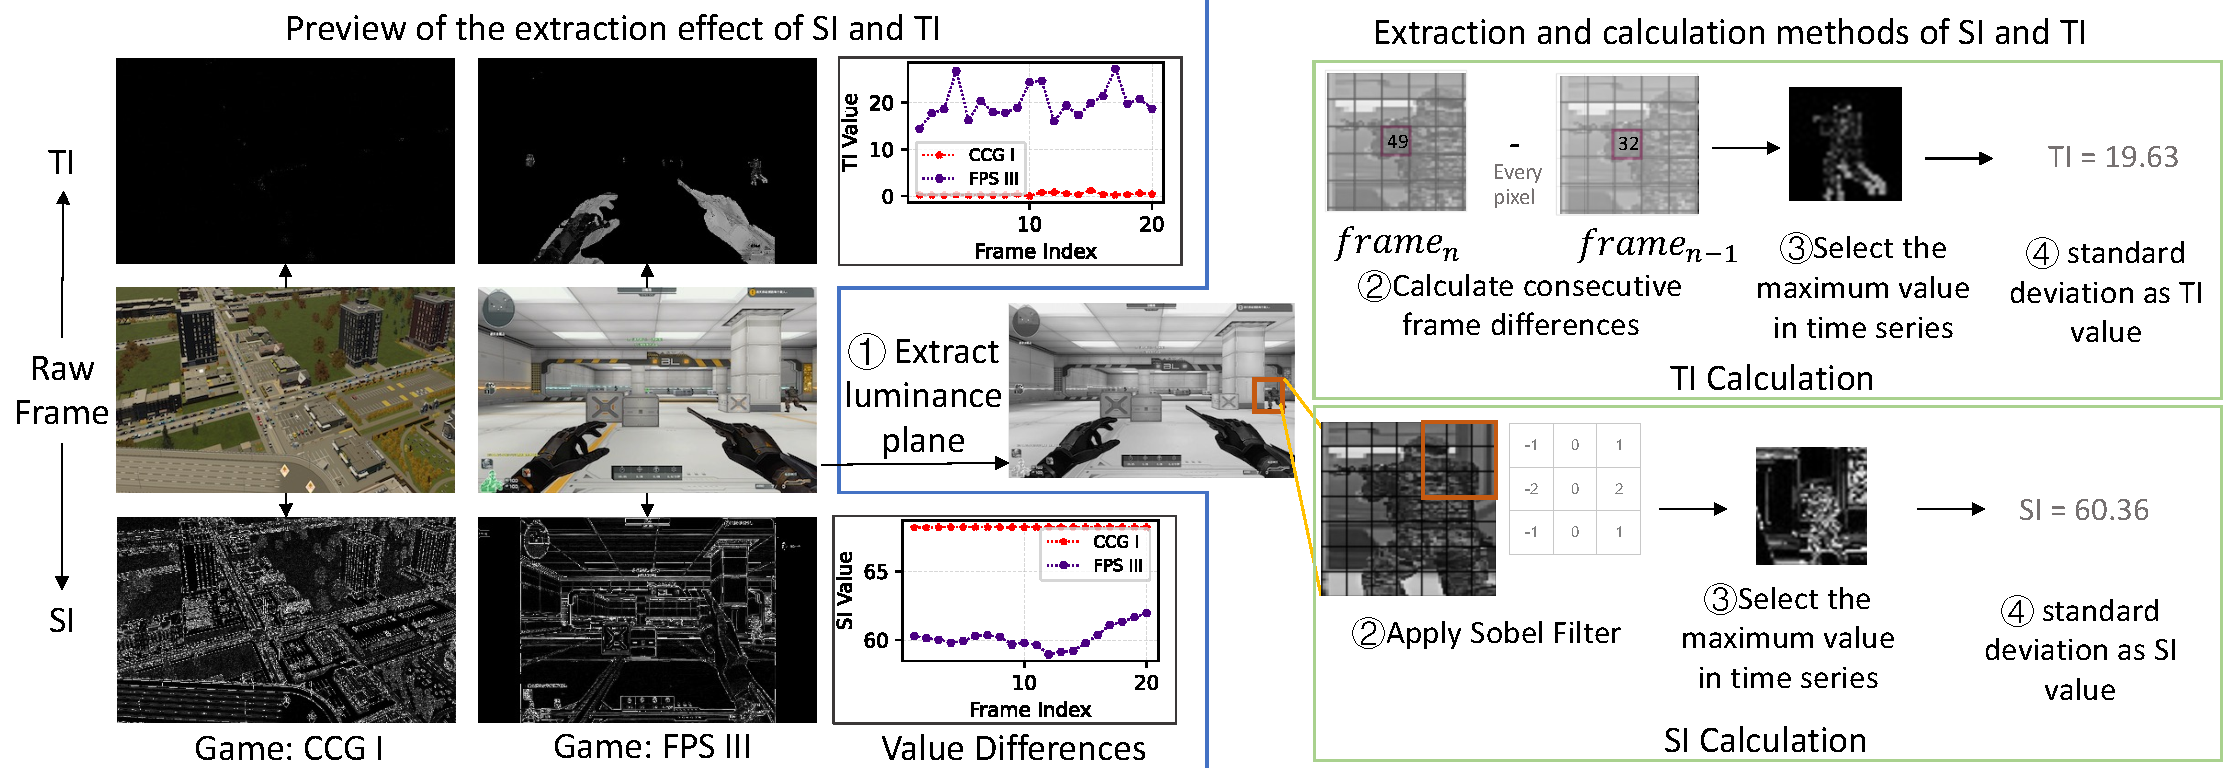
\includegraphics[width=\textwidth]{figures/chap03/intra_schematic_diagram.pdf} 
\caption{两款不同视频游戏的TI和SI提取结果的预览}
\label{fig_intra_schematic_diagram}
\end{figure}

图\ref{fig_intra_schematic_diagram}展示了来自两个场景的随机帧,并附有相应的灰度图像,这些图像映射了空间感知信息(SI)和时间感知信息(TI)值。TI 作为内容变化的指示器,使得 CCG I 由于内容变化较小,呈现出主要是黑色的图像。相反,FPS III 由于内容变化显著,展示了明显的视觉差异。SI 作为空间细节的指示器,在应用 Sobel 算子提取灰度图像时,突出了显著的边缘轮廓。特别是在视觉复杂的帧中,如 CCG I,游戏的场景内容相较于 FPS III 显得更为复杂。通过比较两款游戏中 SI 和 TI 的值差异,可以看出 CCG I 的 SI 值高于 FPS III,而 TI 值较低。此外,CCG I 的波动性较小,FPS III 则波动较大。这一观察结果强调了如何通过 SI 和 TI 度量有效捕捉并反映游戏属性和敏感性特征。

然而,SI 和 TI 的统计值并未明确表现出与游戏延迟敏感性之间的单调关系。为了解决这一问题,本章节采用了无监督聚类方法 K-Means,将数据分为三类,每一类分别表示不同程度的延迟敏感性。这种分类是基于数据与已知延迟敏感性游戏的接近程度进行的。

\section{场景需求可感知传输系统实现与部署}
超低延迟实时通信模拟器: OpenNetLab \cite{eo2022opennetlab} 提供了一个基于 AlphaRTC 的开放平台,用于快速验证基于强化学习的实时通信速率控制算法。本实验对 OpenNetLab 的 gym 模拟器进行了修改,使其适应云游戏场景,包括调整了模拟器的端到端延迟范围,以适应超低延迟需求,并增加了对帧间到达时间间隔(Frame Inter-Arrival Time)的测量能力,使得RL代理能够获得云游戏中特有状态信息,以便与 AlphaRTC 系统的常规系统状态反馈进行配合,

部署强化学习算法:本实验基于 Stable-Baselines3 \cite{stable-baselines3} 和 ReCoCo \cite{markudova2023recoco} 构建了强化学习框架。该框架支持快速构建具有自定义空间和动作的 Actor-Critic 算法,并支持低延迟推理。该框架还集成了多种训练策略,可以快速调用以验证其效果。

设置训练参数:对于式\eqref{eq:total_reward} 中的超参数 $\alpha$,本实验从相等权重开始,通过训练和与相应影响因素的平衡来确定最佳参数。对于状态空间中历史状态的长度,本实验参考了 Aurora \cite{markudova2023recoco} 并根据训练奖励的结果进行了微调。

提取 TI 和 SI 信息: 本实验新增了一个 SI 和 TI 计算模块,以从视频流中获取统计信息。基于已知的游戏敏感度类型,本实验进行了离线分类,并选择了相应的敏感度算法。

相关的算法和模拟系统部署在了一台高性能计算服务器上,配备Intel Xeon Silver 4210 CPU @ 2.20GHz,并搭载4张 NVIDIA Tesla V100S GPU显卡。
\section{实验评估方法与实验结果}
\subsection{实验评估方法设计}
数据集:为了评估Sense方法对用户体验质量(QoE)的改进,实验使用了 OpenNetLab 提供的在不同条件下的网络轨迹。这些轨迹包含了异构网络链路类型,包括有线、4G 和 5G,不同的带宽吞吐量条件。具体的链路类型为:有线 - (12Mbps),4G - (3Mbps, 700Kbps, 500Kbps) 和 5G - (35Mbps, 12Mbps, 900Kbps)。这些带宽链路的平均带宽、抖动标准差、带宽变化均值以及可模拟的总时长统计信息如表\ref{tab:bandwidth_variation}所示。

\begin{table}[ht]
    \caption{不同网络条件下的带宽和变化情况}
    % \renewcommand\arraystretch{1}
    \centering
    \resizebox{\columnwidth}{!}{%
    \begin{tabular}{@{}ccccc@{}}
    \toprule
    网络链路 & 平均带宽 (Kbps) & 抖动标准差 (Kbps) & 带宽变化均值 (Kbps) & 总时长 (秒) \\ \midrule
    WIRED\_35Mbps & 35258.76 & 3202.53 & 657.34 & 61.3 \\ 
    5G\_13Mbps   & 17315.63 & 1617.53 & 327.55 & 60.7 \\
    5G\_12Mbps   & 11644.95 & 4663.19 & 399.03 & 61.0 \\ 
    5G\_900Kbps  & 862.67   & 97.20   & 133.98 & 57.6 \\
    4G\_3Mbps    & 3019.52  & 459.90  & 57.06  & 60.8 \\ 
    4G\_700Kbps  & 678.61   & 253.62  & 165.30 & 106.6 \\ 
    4G\_500Kbps  & 497.96   & 200.42  & 124.16 & 106.0 \\ \bottomrule
    \end{tabular}
    }
    \label{tab:bandwidth_variation}
\end{table}

其中具体参数的计算如式\eqref{eq:avg_bandwidth},式\eqref{eq:standard_deri}和式\eqref{eq:deri_band_avg}所示:
\begin{equation}
\begin{aligned}
\text{平均带宽} \mu = \frac{\sum_{i=1}^{n} capacity_i \times duration_i}{\sum_{i=1}^{n} duration_i},
\end{aligned}
\label{eq:avg_bandwidth}
\end{equation}
\begin{equation}
\begin{aligned}
\text{抖动标准差} = \sqrt{\frac{\sum_{i=1}^{n} duration_i \times (capacity_i - \mu)^2}{\sum_{i=1}^{n} duration_i}}
\end{aligned},
\label{eq:standard_deri}
\end{equation}
\begin{equation}
\begin{aligned}
\text{带宽变化均值} = \frac{\sum_{i=1}^{n-1} |capacity_i - capacity_{i+1}| \times duration_i}{\sum_{i=1}^{n-1} duration_i}
\end{aligned}.
\label{eq:deri_band_avg}
\end{equation}
其中,$capacity_i$代表$i$时刻的带宽容量,$duration_i$代表模拟中的时刻$i$。

与基线算法的比较:本章节将Sense算法与 GCC 和 ReCoCo 的 QoE 实验结果进行了比较。

\begin{itemize}
    \item GCC算法 \cite{carlucci2016analysis}:GCC 算法结合了基于丢包的控制器和基于延迟的控制器,是 WebRTC 中默认的速率控制方法。它在低延迟场景下提供了稳定的连接,并能够较好地适应不同的网络状况。
    
    \item ReCoCo \cite{markudova2023recoco}:ReCoCo 是一种利用强化学习技术的拥塞控制算法,能够在复杂网络条件下实现超低延迟优化。
\end{itemize}


性能指标:本章节使用QoE作为衡量最终算法改进的指标。QoE 包括两个方面:延迟和视觉质量。
\begin{itemize}
    \item 延迟:通过MTP延迟 $L_{MTP}$ \cite{alhilal2022nebula} 进行评估,该指标衡量从用户执行操作(如键盘按键或鼠标移动)到操作结果在屏幕上显示所需的帧时间延迟。MTP延迟所对应的QoE分数可以使用式\eqref{eq:expr} 中的延迟感知敏感度函数 $r(d)$ 进行计算。
    
    \item 视觉质量:由流畅度和平滑度组成。流畅度衡量显示帧的连续性,避免因丢包和接收超时导致的帧丢失、冻结或抖动。在固定时间段内屏幕冻结的次数记为 $J$,每次冻结或抖动都会作为 QoE 的惩罚分数。平滑度评估显示帧的量化级别和分辨率,可通过编码比特率计算。通过使用式\eqref{eq:logsend} 将编码比特率 $s$ 归一化到 $[0, 5]$,以确保发送速率和延迟对 QoE 的贡献相等,归一化后的值记为 $R_{slog}(s)$。
\end{itemize}


一段时间内的平均 QoE 可以通过式\eqref{eq:qoeeva}计算:
\begin{equation}
\begin{aligned}
    QoE = 0.5 * r(L_{MTP})  + 5 * R_{slog}(s) - 0.25 * J  .
\end{aligned}
\label{eq:qoeeva}
\end{equation}

游戏敏感性分类通过 K-Means 聚类算法进行评估,并通过分类准确率作为聚类算法的评价指标。

\subsection{用户体验评估实验结果}
总体 QoE 增益:本实验使用式\eqref{eq:qoeeva} 计算了算法的最终 QoE,所有相应的结果列在表\ref{tab:exp_results} 中。

% Please add the following required packages to your document preamble:
% \usepackage{booktabs}
% \usepackage{multirow}
\begin{table*}[!ht]
\caption{Sense的QoE实验结果与其他方法对比}
\resizebox{\linewidth}{!}{%
\begin{tabular}{@{}cccccccccc@{}}
\toprule
网络条件 & 游戏类型分类 & 方法 & 平均延迟 & 尾部延迟 (95\%) & 平均 r($L_{MTP}$) & 平均发送速率(Kbps) & $R_slog(s)$ & 抖动次数 & 最终 QoE \\ \midrule
\multirow{9}{*}{\begin{tabular}[c]{@{}c@{}}高吞吐量\\      ($\geq$ 10Mbps)\end{tabular}} & \multirow{3}{*}{高敏感度} & ReCoCo               & 50.501          & 101.166             & 2.802             & 4748.340               & 4.610    & 6            & 1.728          \\
                                                                                                      &                            & GCC                  & 53.776          & 130.871             & 2.563             & 1926.600               & 3.935    & 3            & 1.687          \\
                                                                                                      &                            & \textbf{Sense(提出方法)} & 50.600          & 102.690             & 2.794             & 4379.535               & 4.549    & 3            & \textbf{1.898} \\ \cmidrule(l){2-10} 
                                                                                                      & \multirow{3}{*}{中敏感度}    & ReCoCo               & 50.501          & 101.166             & 3.739             & 4748.340               & 4.610    & 6            & 1.962          \\
                                                                                                      &                            & GCC                  & 53.776          & 130.871             & 3.621             & 1926.600               & 3.935    & 3            & 1.952          \\
                                                                                                      &                            & \textbf{Sense(提出方法)} & 50.600          & 101.000             & 3.736             & 2795.595               & 4.214    & 1            & \textbf{2.175} \\ \cmidrule(l){2-10} 
                                                                                                      & \multirow{3}{*}{低敏感度}       & ReCoCo               & 50.501          & 101.166             & 4.424             & 4748.340               & 4.610    & 6            & 2.133          \\
                                                                                                      &                            & GCC                  & 53.776          & 130.871             & 4.292             & 1926.600               & 3.935    & 3            & 2.119          \\
                                                                                                      &                            & \textbf{Sense(提出方法)} & 51.726          & 105.333             & 4.376             & 4582.741               & 4.583    & 0            & \textbf{2.490} \\ \midrule
\multirow{9}{*}{\begin{tabular}[c]{@{}c@{}}低吞吐量\\      (\textless 10Mbps)\end{tabular}}     & \multirow{3}{*}{高敏感度} & \textbf{ReCoCo}      & 53.771          & 110.143             & 2.563             & 237.945                & 2.371    & 4            & \textbf{1.234}          \\
                                                                                                      &                            & GCC                  & 177.772         & 1277.680            & 1.000             & 186.950                & 2.190    & 2            & 0.923          \\
                                                                                                      &                            & Sense(提出方法)          & 66.761          & 210.250             & 1.720             & 277.849                & 2.487    & 3            & 1.114          \\ \cmidrule(l){2-10} 
                                                                                                      & \multirow{3}{*}{中敏感度}    & ReCoCo               & 53.771          & 110.143             & 3.622             & 237.945                & 2.371    & 4            & 1.498          \\
                                                                                                      &                            & GCC                  & 177.772         & 1277.680            & 1.000             & 186.950                & 2.190    & 2            & 0.923          \\
                                                                                                      &                            & \textbf{Sense(提出方法)} & 60.397          & 111.000             & 3.373             & 271.060                & 2.468    & 2            & \textbf{1.585} \\ \cmidrule(l){2-10} 
                                                                                                      & \multirow{3}{*}{低敏感度}       & \textbf{ReCoCo}      & 53.771          & 110.143             & 4.292             & 237.945                & 2.371    & 4            & \textbf{1.666}          \\
                                                                                                      &                            & GCC                  & 177.772         & 1277.680            & 1.000             & 186.950                & 2.190    & 2            & 0.923          \\
                                                                                                      &                            & Sense(提出方法)          & 67.640          & 220.200             & 3.533             & 230.204                & 2.346    & 2            & 1.595          \\ \bottomrule
\end{tabular}
}
    \label{tab:exp_results}
\end{table*}

实验结果分别展示了高带宽链路和低带宽链路下的结果,因为云游戏通常更倾向于使用高带宽连接。对于具有不同延迟敏感度的游戏,根据其相应的敏感度曲线绘制 QoE 结果。本章的方法与 GCC 和另一种基于强化学习的方法 ReCoCo 进行了比较。在高敏感度游戏中,本章节提出的方法在延迟方面优于 GCC,并且相比 ReCoCo 方法,虽然延迟略高,但对 QoE 的影响可以忽略不计。这种改进显著减少了屏幕卡顿的发生,从而提高了 QoE 得分。

\begin{table}[!ht]
\centering
\caption{游戏的 SI 和 TI 使用 K-Means 方法进行分类的结果}
\renewcommand\arraystretch{1.25}
\begin{tabular}{@{}ccccc@{}}
\toprule
游戏 & TI & SI & K-means分类 & 正确分类 \\ \midrule
3D-RPG I           & 8.10  & 48.73  & 高敏感度          & 是                    \\
TPS I              & 18.42 & 55.39  & 高敏感度          & 是                    \\
\textbf{FPS III}   & 18.22 & 67.94  & 高敏感度          & 是                    \\
FPS IV             & 17.69 & 71.55  & 高敏感度          & 是                    \\
\textbf{FPS II}    & 16.55 & 72.05  & 高敏感度          & 是                    \\
\textbf{CCG I}     & 2.12  & 74.63  & 低敏感度           & 是                    \\
Sport III          & 11.29 & 77.00  & 低敏感度           & 否 (中敏感度)                   \\
3D-RPG II          & 10.31 & 80.21  & 低敏感度           & 是                    \\
A-RPG I            & 4.03  & 81.97  & 低敏感度           & 是                    \\
MMORPG II          & 14.02 & 84.21  & 低敏感度           & 是                    \\
MMORPG I           & 21.34 & 86.12  & 低敏感度           & 是                    \\
\textbf{MOBA I}    & 3.40  & 87.00  & 低敏感度           & 是                    \\
\textbf{MOBA II}   & 3.74  & 87.51  & 低敏感度           & 是                    \\
FPS I              & 27.74 & 89.25  & 低敏感度           & 否 (高敏感度)
                        \\
Casual III         & 10.73 & 91.49  & 中敏感度          & 是                    \\
Casual II          & 8.39  & 92.64  & 中敏感度          & 是                    \\
\textbf{Sport I}   & 11.76 & 103.32 & 中敏感度          & 是                    \\
\textbf{2D-RPG I}  & 8.13  & 108.18 & 中敏感度          & 是                    \\
\textbf{2D-RPG II} & 17.33 & 119.28 & 中敏感度          & 是                    \\ \bottomrule
\end{tabular}
\label{tab_cat_gor}
\end{table}

场景敏感度分类: 本实验通过分析游戏平台上每款游戏的动态视觉效果,对 19 款游戏进行了测试。对于每款游戏大约 600 秒的数据,实验逐帧计算了 SI(空间信息)和 TI(时间信息)值,并求取其平均值。基于 SI 和 TI 的平均值,实验使用 K-Means 方法 \cite{ahmed2020k} 进行了聚类。分类结果如表\ref{tab_cat_gor}所示。对于剩余的游戏,实验基于先前测量的游戏作为基准,确定了最终的敏感度标签。在 19 款游戏和场景中,分类结果显示仅有两款游戏的敏感度标签不匹配,分类准确率达到了 89.4\%。






训练过程中的奖励函数累计值及运行性能如图\ref{fig-evaluation-result}所示。图\ref{fig-reward-func}显示了训练过程中累计奖励的变化。图\ref{fig-band-util}、\ref{fig-latency-cdf}和\ref{fig-jitter-times}展示了算法运行过程中收集的状态参数。图\ref{fig-band-util}显示了在相同带宽下发送速率的变化,结果表明Sense算法与 ReCoCo 相似,并且超越了 GCC。图\ref{fig-latency-cdf}显示了数据包延迟的累积分布函数(Cumulative Distribution Function,CDF),高敏感度和中敏感度的低延迟表现优于 ReCoCo,而低敏感度则保持在不敏感范围内。图\ref{fig-jitter-times}展示了Sense算法在固定时间段内能实现更少的抖动次数。

\begin{figure}[!ht]
\centering
\begin{subfigure}[t]{0.5\linewidth}
  \centering
  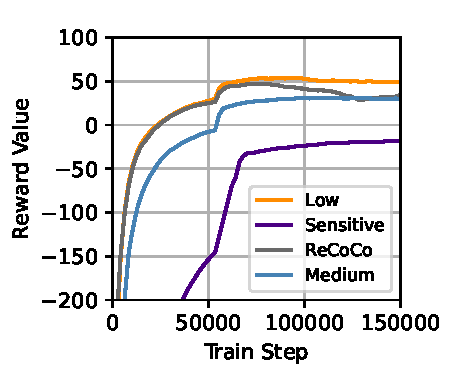
\includegraphics[width=\linewidth]{figures/chap03/evaluation_plots/reward_value.pdf}
  \caption{训练过程中的奖励值累计}
  \label{fig-reward-func}
\end{subfigure}%
\begin{subfigure}[t]{0.5\linewidth}
  \centering
  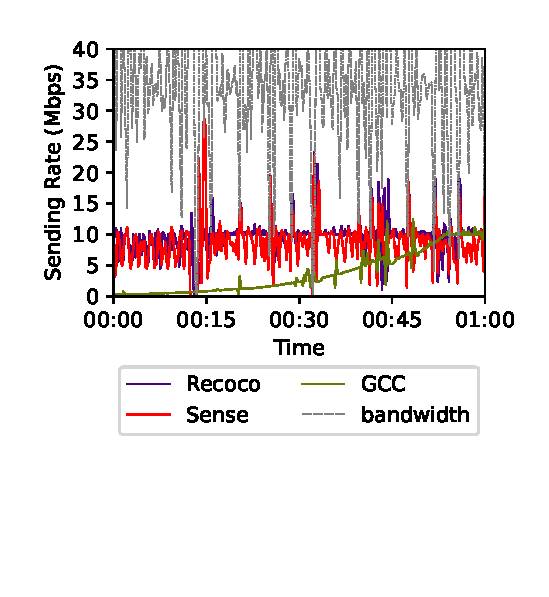
\includegraphics[width=\linewidth]{figures/chap03/evaluation_plots/bandwidth.pdf}
  \caption{带宽利用率}
  \label{fig-band-util}
\end{subfigure}

\begin{subfigure}[t]{0.5\linewidth}
  \centering
  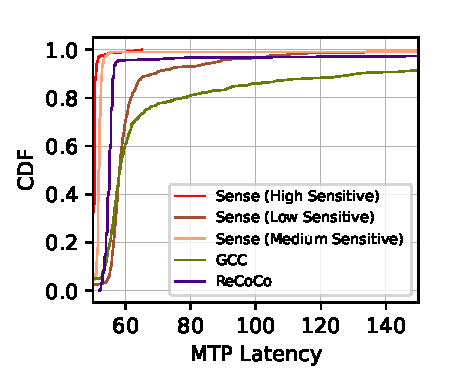
\includegraphics[width=\linewidth]{figures/chap03/evaluation_plots/cdf_delay.pdf}
  \caption{延迟的累积分布函数 (CDF)}
  \label{fig-latency-cdf}
\end{subfigure}%
\begin{subfigure}[t]{0.5\linewidth}
  \centering
  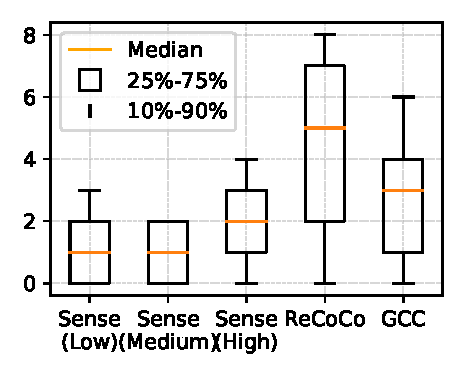
\includegraphics[width=\linewidth]{figures/chap03/evaluation_plots/jitter_times.pdf}
  \caption{抖动次数}
  \label{fig-jitter-times}
\end{subfigure}

\caption{训练过程中的奖励函数累计值及运行性能}
\label{fig-evaluation-result}
\end{figure}

 

\subsection{设计方案局限性讨论}
如果一款游戏场景被错误分类,将会对性能带来怎样的影响?为了进一步分析错误分类对系统性能的影响,本实验继续进行了两个案例研究,分别探讨高敏感度场景被误分类为低敏感度以及低敏感度场景被误分类为高敏感度时的 QoE 变化情况。实验结果如表\ref{miscals}所示。如果高敏感度场景被误分类为低敏感度,会导致显著的 QoE 损失,几乎抵消了 Sense 的优势;但若低敏感度场景被误分类为高敏感度,导致“过度满足”的延迟 QoE,但略微降低了图像质量并增加了卡顿。尽管这些情况的发生会降低QoE,但最差的结果也不会低过最低基准能够达到的QoE;且这些是极端的误分类情况,第一个案例代表了最差的结果。这些情况发生的概率也非常罕见。
\begin{table}[ht]
\centering
\caption{敏感度误分类对QoE的影响}
\renewcommand\arraystretch{1.25}
\resizebox{\columnwidth}{!}{%
\begin{tabular}{@{}cccc@{}}
\toprule
\textbf{案例} & \textbf{QoE} & \textbf{相较于正确分类的 QoE} & \textbf{相较于最低基准的 QoE} \\ \midrule
应为高敏感度但被误分类为低敏感度 & 1.84  & -7.43\%                     & +0.54\%                     \\ 
应为低敏感度但被误分类为高敏感度 & 2.30  & -0.90\%                     & -0.04\%                     \\ \bottomrule
\end{tabular}
}
\label{miscals}
\end{table}

\section{本章小结}
本章节提出了 Sense,一种基于强化学习的用户时延敏感度可感知的场云游戏场景传输速率控制算法。通过测量和用户 MOS 实验,利用不同游戏在延迟感知敏感度上的差异,Sense 在强化学习框架中重构了状态和奖励空间。这使得可以根据游戏敏感度的不同类别,对延迟和视觉质量权衡采取差异化策略。实验结果表明,Sense 提高了视频流的流畅性,将总体用户体验质量(QoE)提升了 9.8\% 至 16.7\%,并以 89.4\% 的准确率完成了游戏敏感度分类。
















